\documentclass[a4paper]{article}

\usepackage[english]{babel}
\usepackage[utf8]{inputenc}
\usepackage{amsmath}
\usepackage{graphicx}
\usepackage{placeins}
\usepackage{float}

\usepackage[colorinlistoftodos]{todonotes}
\usepackage{titling}
\setlength{\droptitle}{-4.5cm}
\usepackage{amssymb}
\usepackage{algorithm,algpseudocode}
\usepackage{subfig}
\usepackage{bm,nicefrac}
\usepackage{comment}
\usepackage{authblk}
\usepackage{tikz}
\usepackage{float}

\usepackage{amsthm}
 
\renewcommand\qedsymbol{$\blacksquare$}

\newtheorem{mydef}{Definition}
\newtheorem{myremark}{Remark}

\usepackage{hyperref}
\hypersetup{
    colorlinks=true,
    linkcolor=blue,
    filecolor=magenta,      
    urlcolor=cyan,
}


\title{Parallelized calculation of permutation tests}
\author[1]{Markus Ekvall}
\author[2]{Michael H\"{o}hle}
\author[1]{Lukas K\"{a}ll}
\affil[1]{Science for Life Laboratory, School of Engineering Sciences in Chemistry, Biotechnology and Health,
 KTH -- Royal Institute of Technology, Box 1031, 171~21 Solna, Sweden}
 \affil[2]{Department of Mathematics, Stockholm University,
  106~91 Stockholm, Sweden}

\addtolength{\textwidth}{1.8cm}

\begin{document}
%\tableofcontents
\maketitle

\begin{abstract}
Permutation tests offers a straight forward framework to assess the siggnificance of difference in sample statistics. A major advantage of permutation tests are the relatively few assumptions about the distribution of the test statistic are needed, as they rely on the assumption of exchangability of the group labels. They have great value, as they allow a sensitivity analysis in order to determine to what extend the assumed large sample distribution of the test statistic applies. However, in this situation permutation tests are rarely applied, because the running time of naive implementations is too slow and grows exponentially with the sample size. Nevertheless, continued development in the 1980s introduced dynamic programming algorithms that computes exact permutation tests in polynomial time. Albeit this significant run time reduction, the exact test have not yet become one of the predominant statistical tests for medium sample size. In this paper we propose a computational parallelization refinement of permutation tests, which could  help make permutation test more attractive. Parallelization is possible by nontrivial rearrangement of the structure of the algorithm. Making the computation parallel on a GPU gains additional orders of magnitude of speedup of this algorithm. Here we demonstrate an implementation of exact permutation tests, for which the execution time would essentially become a non-issue for sample sizes up to X samples. \todo[inline]{Say something or refer to an example or a situation, where this approach is particularly useful? Furthermore, one probably has to say a little bit more about when the large sample situation applies.}
\end{abstract}

\section{Introduction}
Permutation tests are frequently used for non-parametric testing and are especially valuable within computational biology, with applications within genome wide association studies \cite{purcell2007plink,browning2008presto,dudbridge2008estimation}, Pathway Analysis\cite{subramanian2005gene,jeuken2018simple}, and expression quantitative trait loci studies\cite{doerge1996permutation, sul2015accurate}. 
Permutation tests can roughly be divided into Monte Carlo-based sampling techniques\cite{segal2018fast}, and exact tests that derive full permutation distributions.

Exact tests are traditionally seen as unattractive for larger sample sizes, as the number of permutation grows super-exponentially with the sample size. Nonetheless, such computational problems were partially overcome by a theorem by \cite{pagano_trichtler1983}, and inspired a dynamic programming algorithm that has been made explicit by \cite{zimmermann1985}. This algorithm is effective compared with any naive approach, however, the popularity of the exact test for larger set sizes has not attracted much attention the latest coupe of decades. Here we studied the properties of a Graphics processing unit (GPU) implementation of parallelized implementation of such an exact test, and found it superior to the other tested alternatives in terms of speed and accuracy. The outline of this study is as follows, firstly, the main objective–how to perform hypothesis testing with an exact test–is described in section \ref{sec:PvalueComputation}, a detailed explanation of the algorithm is presented in section \ref{sec:calcBottleneck}, a further description how this algorithm can be parallelizable is presented in section \ref{sec:paraAlgo}, and, finally, the result section \ref{sec:result}, comparing the empirical runtimes between the non-parallelized version and parallelized version.

\section{Hypothesis testing}
\label{sec:PvalueComputation}


Let $\bm{x}^A=(x_1^A,\ldots, x_m^A)$ and $\bm{x}^B=(x^B_1,\ldots,x^B_n)$ be two independent non-negative integer valued samples from the distributions $\mathcal{D}(\mu^A)$ and $\mathcal{D}(\mu^B)$ with population means $\mu^A$ and $\mu^B$, respectively. So, $x^A_i \stackrel{\text{iid}}{\sim} \mathcal{D}(\mu^A),$ and $x^A_i \in \mathbb{N}_0$ for $1\leq i \leq m$; and $x^B_i \stackrel{\text{iid}}{\sim} \mathcal{D}(\mu^B),$ and $x^B_j \in \mathbb{N}_0$ for $1\leq j\leq n$. We also form the concatenation of the samples as $\bm{x}=(x^A_{1},\ldots,x^A_{m},x^B_{1},\ldots,x^B_{n})=(x_1, x_2, \ldots, x_{n+m})$.
Our interest is in investigating the hypothesis $H_0: \mu^A = \mu^B$ vs. the alternative $H_A: \mu^A > \mu^B$. Note that we without loss of generality write the null-hypothesis as a point-hypothesis. If one instead has a composite null hypothesis of the type $H_0: \mu^A \leq \mu^B$, the procedure is to conduct the test under the most extreme parameter value of the null-hypothesis, which (for all relevant problems) is $\mu^A = \mu^B$~\cite[Sect. 5.9]{lehmann2008testing} and the test thus corresponds to the point-hypothesis case.

A way to perform the test is to determine how extreme the observed sum of sample $\bm{x}^A$, $s_{\text{obs}} = \sum_{i=1}^m x^A_i$ is under the null hypothesis $H_0: \mu^A = \mu^B$. Typically, this is done under the assumption of a particular parametric family of distributions for both null and alternative, which are parametrized by their respective mean parameters. One then conducts the test by computing the $p$-value
as the probability to observe $s_{obs}$ or a more extreme value in the direction of the alternative under the assumption that the null-hypothesis is true. However, it is rarely possible to compute this probability analytically and one often has to resort to asymptotic approximations. A non-parametric permutation test approach to the testing problem is to instead assume exchangability of the labels $A$ and $B$ under $H_0$, and calculate how frequently samples with sample sums greater or equal than $s_{obs}$ appears when resampling from $\bm{x}$. 
\todo[inline]{MH: Should we provide some reference to what this test is called. Is this the Wilcox test? LK: I am not sure what a Wilcox test is. Is that the same thing as a Wilcoxon signed-rank test? I would (weakly) prefer either ``permutation test'' or ``exact test''.}

We can formulate the $p$-value as, $\Pr(s_{\text{obs}} \leq S | \bm{x},H_0)$, where $\Pr(S| \bm{x},H_0)$ is the probability mass function and $S$ is a random variable denoting the value of the sum in the first sample under the permutation distribution. The computationally expensive part is to obtain $\Pr(S)$ which is estimated by concatenating $\bm{x}^A$ and $\bm{x}^B$ to $\bm{x}=(x^A_{1},\ldots,x^A_{m},x^B_{1},\ldots,x^B_{n})=(x_1, x_2, \ldots, x_{n+m})$, and draw all possible subsets of length $m$ from $\bm{x}$ and count the number of occurrences of all possible sums; when the numbers of occurrences of all possible sums are available, the distribution is accessible. This notion of subset is needed for further reasoning, and hence worth an explicit definition.

\begin{mydef} A set $\bm{z}$ is a cardinality-$j$ subset of a set $\bm{x}$ if it is a subset of $\bm{x}$ with $j$ distinct elements, i.e. $\bm{z} \subseteq \bm{x} \land |\bm{z}|=j$ .\end{mydef}

\begin{mydef} $\mathcal{P}_{=j}(\bm{x})$ is the set of all cardinality-$j$ subsets of a set $\bm{x}$.\end{mydef}

\begin{mydef} $\mathcal{P}^s_{=j}(\bm{x})$ is the set of all cardinality-$j$ subsets with elements that sum to $s$ of a set $\bm{x}$, i.e. $\mathcal{P}^s_{=j}(\bm{x})=\{  \bm{z} \mid \forall \bm{z}\in \mathcal{P}_{=j}(\bm{x}) \land \sum_{e \in \bm{z}}e=s \}$.\end{mydef}

The maximal sum obtained from a cardinality-$m$ subsets of $\bm{x}$ is $s_{\rm max}$ (i.e., a subset containing the $m$ largest values in $\bm{x}$); hence, the possible states of the integer sum of any cardinality-$m$ subsets are $\Omega=\{0,1,\ldots,s_{\rm max}\}$ (recall that $x_{i}\in \mathbb{N}_0$ ), which denotes the support of the sum. Assume a random variable $\bm{x}^{*}=(x^{*}_1,\ldots,x^{*}_m)$, that is a randomly sampled cardinality-$m$ subset from $\bm{x}$ and its corresponding sum is $S=\sum_{i=1}^m x^{*}_i$, where $S\in \Omega$. Then $\Pr(S)$ can be expressed as the fraction of cardinality-$m$ subsets that sum to $s$ out of all cardinality-$m$ subsets of $\bm{x}$.

\begin{align}
\label{eq:pOfS}
\Pr(s) = \Pr(S = s) = \frac{|\mathcal{P}^s_{=m}(\bm{x})|}{|\mathcal{P}_{=m}(\bm{x})|},
\end{align}

where $0\leq s \leq s_{\rm max}$. From basic combinatorics the denominator of the above equation \ref{eq:pOfS} is equal to:

\begin{align*}
{m+n \choose m} = \frac{(m+n)!}{n!m!}
\end{align*}

The calculation of the numerator is the intricate part (e.g., a naive algorithm that would exhaustively check the sum for each possible cardinality-$m$ subsets and compare it to $s$, for all $s$, would take $\mathcal{O}(s_{\rm max} \cdot {m+n \choose m})$, i.e., a combinatorial explosion) and how to set-up an efficient algorithm with polynomial time complexity is further discussed in section \ref{sec:calcBottleneck}. However, for the sake of discussion, here is the definition of the general case of the numerator.

\begin{mydef}
\label{def:numerator}
$N(s,j)=|\mathcal{P}^s_j(\bm{x})|$, i.e. the number of cardinality-$j$ subsets of a set $\bm{x}$ s.t. their elements sum is equal to $s$.
\end{mydef}

By definition \ref{def:numerator}, the specific numerator in equation \ref{eq:pOfS} is then $N(s,m)$, and when attained, the sought $p$ value can be calculated as:

\begin{align}
\Pr(s_{\text{\rm obs}} \leq S | \bm{x}) &= \sum _{s=s_{\rm obs}}^{s_{\rm max}}\frac{N(s,m)}{{m+n \choose m}}=\sum _{s=s_{\rm obs}}^{s_{\rm max}}\Pr(s)
\end{align}

Alternatively, we can use the same framework to calculate the mid $p$ value \cite{routledge1994practicing} as, 

\begin{align}
p_{\rm mid}(s_{\rm obs}) &= \frac{1}{2}\Pr(s_{\rm obs}) +\sum _{s=s_{\rm obs}+1}^{s_{\rm max}}\Pr(s).
\end{align}

As mentioned above, there is no trivial method to obtain $N(s,m)$. However, it is possible to develop a  dynamic programming algorithm to obtain $N(s,m)$ \cite{pagano_trichtler1983, zimmermann1985}, which is described thoroughly in the next section.

\section{Dynamic programming: Efficient calculation of $N(s,m)$}
\label{sec:calcBottleneck}

A dynamic programming algorithm for calculating $N(s,m)$ was first implemented and proved by \cite{zimmermann1985, pagano_trichtler1983}. Therefore, the correctness of the algorithm is not under scrutiny in this section. However, we here give a walk-through of the algorithm, and subsequently describe its parallelization in section \ref{sec:paraAlgo}.

We would like to find a recursive relation between $N(s,m)$ and a simpler case of itself. One such relation is offered by considering fewer elements of $\bm{x}$. Let's consider the case where we calculate $N(s,j)$ for a the subset of the $k$ first $x_i$'s, i.e. $\{ x_h \}^i_{h=1}$, by first defining the cardinality-$j$ subsets for this truncated $\bm{x}$ set. 

\begin{mydef}
\label{def:specificNumerator}
\begin{align*}
N(s,i,j)&= |\mathcal{P}^s_j(\{ x_h \}^i_{h=1})|
\end{align*}
\end{mydef}
\begin{myremark}
\label{rm:finalN}
For a set $\bm{x}$ such that $|\bm{x}|=k$, then $N(s,i=k,j)=N(s,j)$, since $\{ x_h \}^k_{h=1}=\bm{x}$, hence, definition \ref{def:numerator} and definition \ref{def:specificNumerator} are compatible.
\end{myremark}

It follows directly from definition \ref{def:specificNumerator} that we can not select subsets of $\bm{x}$ with fewer elements than required to form a cardinality-$j$ subsets, i.e. when $i<j$. Also, $N(s,i,j)$ has to be zero when either $i=0$ (i.e., checking the empty set of $\bm{x}$), when $s < 0$, or when $s_{\rm max} < s$ (i.e., when $s$ is outside the boundary of possible sums). Hence, 

\begin{align}
\label{eq:boundryCondition1}
N(s,i,j) &=0, & \text{if $i < j$, $i=0$, $s < 0$, or $s_{\rm max} < s$.}
\end{align}

Also, the empty set $\emptyset$ trivially reach the sum $s=0$, thus

\begin{align}
\label{eq:boundryCondition2}
N(s,i,j) &= 1 & \text{if $j=s=0$.}
\end{align}

Equation \ref{eq:boundryCondition1} and \ref{eq:boundryCondition2} will later form the base case for the algorithm.

The expression of $N(s,i,j)$ in definition \ref{def:specificNumerator} is not yet especially helpful, but since it is possible to consider fewer elements of $\bm{x}$, it is possible to re-factoring the expression. To do so we first define 
\begin{mydef}
\label{def:specificNumerator2}
$\phi (s,i,j)$ is the number of cardinality-$j$ subsets containing an element $x_i$ with elements that sum to $s$ of a set $\{ x_h \}^i_{h=1}$, i.e. $\phi (s,i,j)=|\{ \bm{a} \mid \bm{a}\in \mathcal{P}^s_j(\{ x_h \}^i_{h=1}) \land x_i \in \bm{a} \}|$.\end{mydef}


This allows us to form a recursion of $N(s,i,j)$ as,
\begin{align}
\label{eq:recursion1}
N(s,i,j) &= |\mathcal{P}^s_j(\{ x_h \}^i_{h=1})| = \\
    &= |\mathcal{P}^s_j(\{ x_h \}^{i-1}_{h=1})| 
    + |\{ \bm{a} \mid \bm{a}\in \mathcal{P}_j(\{ x_h \}^i_{h=1}) \land \sum_{e \in \bm{a}}e=s \land x_i \in \bm{a} \}| = \\
    &= N(s,i-1,j)+ \phi (s,i,j).
\end{align}


\begin{comment}


Before the recursion becomes practically amendable we need a method to efficiently calculate $\phi (s,i,j)$. This function $\phi (s,i,j)$ will differ for cardinality-$j$ subsets with one element (i.e., $j=1$.), and those with more elements (i.e., $j>1$.). Here is a formal description of the first case (i.e., $j=1$.) Since there is only one element in a $1$-subset, then either $x_{i}=s$ or it is not. Thus,

\begin{align}
\label{eq:cond3}
\phi (s,i,j=1) &=\begin{cases}
    1, & \text{if $j=1$ and $x_{i}=s$}.\\
    0, & \text{if $j=1$ and $x_{i}\neq s$}.
  \end{cases}
\end{align}

\todo[inline]{@ME: Is it not more natural to define N(0,0,0)=1, and get rid of eq \ref{eq:cond3}?}

Combine the recursive form \ref{eq:recursion1} with condition \ref{eq:cond3} to obtain the sub-recursion below:

\begin{align}
\label{eq:Subrecursion2}
N(s,i,j) &=\begin{cases}
    N(s,i-1,j)+1, & \text{if $j=1$ and $x_{i}=s$}.\\
    N(s,i-1,j), & \text{if $j=1$ and $x_{i}\neq s$}.
  \end{cases}
\end{align}

\end{comment}


Here is an example, to of the usage of $\phi (s,i,j)$, to build up some intuition: Say that the only $2$-subsets summing up to $5$ are $\{2,3\}$ and $\{0,5\}$ in $x[1,\ldots,4]$, and hence $N(5,4,2)=2$ (see definition \ref{def:specificNumerator}). Furthermore, when extending $x[1,\ldots,5]$ where $x_{5}=5$, by the assertion in the previous line, the only $3$-subsets summing up to $10$ that contains $x_{5}$ is $\{2,3\} \cup {x_{5}}$ and $\{0,5\} \cup {x_{5}}$, and therefore $\phi (10,5,3)=2$ (see definition \ref{def:specificNumerator2}). The crucial observation is that there is an equivalence $\phi (10,5,3)=N(5,4,2)$ .

For the general case, say that $N(s - x_{i},i-1,j-1)$ is known. Thus, by adding $x_{i}$ to all those $(j-1)$-subsets summing up to $(s - x_{i})$ counted by $N(s - x_{i},i-1,j-1)$, the number of cardinality-$j$ subsets summing up to $s$ that contains $x_{i}$ which $\phi (s,i,j)$ ought to count is revealed–namely $N(s - x_{i},i-1,j-1)=\phi (s,i,j)$, given $x_{i} \leq s$, since there exist no $s<0$.
\begin{align}
\label{eq:cond4}
\phi (s,i,j) &=\begin{cases}
    N(s - x_{i},i-1,j-1), & \text{if $j>0$ and $x_{i} \leq s$}.\\
    0, & \text{if $j>0$ and $s < x_{i}$}.\\
  \end{cases}
\end{align}

Again, we combine the recursion \ref{eq:recursion1} with the condition \ref{eq:cond4} to obtain the generic sub-recursion below.

\begin{align}
\label{eq:Subrecursion3}
N(s,i,j) &=\begin{cases}
    \text{$N(s,i-1,j)$ + $N(s-x_{j},i-1,j-1)$}, & \text{if $j>0$ and $x_{i} \leq s$}.\\
    \text{$N(s,i-1,j)$}, & \text{if $j>0$ and $s < x_{i}$}.\\
  \end{cases}
\end{align}

By combining the base case \ref{eq:boundryCondition1} and \ref{eq:boundryCondition2} with the generic sub-recursion \ref{eq:Subrecursion3}, the final recursion is:

\begin{align}
\label{eq:finalRecursion}
\text{$N(s,i,j)$}   =\begin{cases}
    1, & \text{if $j=s=0$.} \\
    0, & \text{if $i < j$, $i=0$, and $s < 0$.} \\
    \text{$N(s,i-1,j)$ + $N(s-x_{j},i-1,j-1)$}, & \text{if $j>0$ and $x_{i} \leq s$}. \\
    \text{$N(s,i-1,j)$}, & \text{if $j>0$ and $s < x_{i}$}. \\
  \end{cases}
\end{align}

\FloatBarrier
\begin{algorithm}
\caption{\# cardinality-$j$ subsets s.t. their elements sum is equal to $s$.}

\label{alg:combination}
\begin{algorithmic}[1]
\State $m$: Scalar equal to the number of samples in $x^{A}$.
\State $n$: Scalar equal to the number of samples $y$.
\State $s_{\rm max}$: Scalar equal to the sum of the $m$ largest values in $x$.
\State $x$: Concatenated vector of $x^{A}$ and $y$ with length $m+n$.
    \Procedure{NumberOfSubsets}{$m$, $n$, $s_{\rm max}$, $x$}
    \State $x=[0 ]+x$ \Comment{Include the empty set $\emptyset$ to $x$}
    \State $m=m+1$ \Comment{Correct the indices for this inclusion.}
    \State Allocate array $N_{old}[0...s_{\rm max},0...m]$ with zeros
    \State Allocate array $N_{new}[0...s_{\rm max},0...m]$ with zeros
    \For{$i=1$ to $(m + n) +1$}
        \For{$j=1$ to $m+1$}
            \For{$s=0$ to $s_{\rm max} +1$}
                \If{$s=(j-1)=0$} \Comment{Sub-recursion \ref{eq:boundryCondition2}} \State $N_{new}[s,j-1]=1$
                \ElsIf{$i < j$} \Comment{Sub-recursion \ref{eq:boundryCondition1}} \State $N_{new}[s,j-1]=0$
                \ElsIf{$j>1$ and $x[i-1] \leq s$} \Comment{Sub-recursion \ref{eq:Subrecursion3} } \State $N_{new}[s,j-1]=N_{old}[s-x[i-1],j-2] + N_{old}[s,j-1]$
                \ElsIf{$j>1$ and $x[i-1] > s$} \State $N_{new}[s,j-1]=N_{old}[s,j-1]$
                \EndIf
            \EndFor
        \EndFor
        \State $N_{old} = N_{new}$; \Comment{Update $N_{old}$ for next iteration.}
    \EndFor
        \State \Return $N_{new}[0...s_{\rm max},m]$ \Comment{By remark \ref{rm:finalN}: $N_{m+n}[s,m]=N(s,m)$}

    \EndProcedure
\end{algorithmic}
\end{algorithm}
\FloatBarrier

The pseudo code of the top-down dynamic programming code of the recursion in Equation \ref{eq:finalRecursion} is given in Algorithm \ref{alg:combination}. The algorithm needs some explanation. Instead of using one extensive array $N[0\ldots s_{\rm max},$\ $0\ldots(m+n),0\ldots m]$, two smaller arrays, $N_{old}[0...s_{\rm max},0...m]$ and $N_{new}[0...s_{\rm max},0...m]$, are swapped and rewritten in each iteration of $i$ in an oscillatory fashion --- to save memory, see line $24$. It is the complete rewriting of $N_{new}$ in the next iteration that makes this possible (any of the conditions in the recursion relation will re-calculate each entry $N_{new}$).

By just keeping $N_{new}$ and $N_{old}$, instead of the full three dimensional array, we save quite some memory. The former two arrays require $\mathcal{O}(s_{\rm max} \cdot m + s_{\rm max} \cdot m) = \mathcal{O}( 2 \cdot s_{\rm max} \cdot m)=\mathcal{O}(s_{\rm max} \cdot m)$, whereas the latter array requires $\mathcal{O}(s_{\rm max} \cdot (m+n) \cdot m)$. Moreover, this improvement in memory usage is a quintessential difference for the parallelized algorithm (the memory storage of the GPU can easily be a bottleneck).

A second point, notice the structure of the for-loops; they could easily have been arranged in whatever way and still obtain correct computations. However, the dimensions of the two arrays have to be adjusted appropriately related to the outer-most loop. Nevertheless, this specific order has a purpose, it is parallelizable --- which will be described in the next section.

One final note on algorithm \ref{alg:combination}, by plain observation on the nested loops, it easy to see that the runtime is $\mathcal{O}(m\cdot (m+n)\cdot s_{\rm max})$.

Here's a demonstration of one iteration of $i$, to make the mechanics of algorithm \ref{alg:combination} even clearer.

\begin{figure}[H]
\centering
\begin{tikzpicture}[set style={{help lines}+=[dashed]}, xscale=1.7, yscale=0.75]
\draw[style=help lines] (0,1) grid +(3,5);
\draw                   (0,5) grid +(1,1);
\node  at  (0.5, 5.5) {$N_{old}(0,0)$};


\draw                   (1,3) grid +(1,1);
\node  at  (1.5,3.5) {$N_{old}(2,1)$};

\draw                   (2,1) grid +(1,1);
\node  at  (2.5,1.5) {$N_{old}(4,2)$};

\draw                   (2,5) grid +(1,1);
\node  at  (2.5,5.5) {$N_{old}(0,2)$};


%
\draw[style=help lines] (4,1) grid +(3,5);
\draw                   (5,3) grid +(1,1);
\node  at  (5.5,3.5) {$N_{new}(2,1)$};

\draw                   (4,5) grid +(1,1);
\node  at  (4.5,5.5) {$N_{new}(0,0)$};
\draw                   (6,1) grid +(1,1);
\node  at  (6.5,1.5) {$N_{new}(4,2)$};

\draw                   (6,5) grid +(1,1);
\node  at  (6.5,5.5) {$N_{new}(0,2)$};


%------------------------------------------------------
% red1
\draw   [red,very thick,dashed,->]   (3,5.5) -- (6,5.5);
\draw   [red,very thick,->]   (1,5.5) -- (5,3.5);
\draw   [red,very thick,->]   (2,3.5) -- (5,3.5);
\draw   [red,very thick,->]   (3,1.5) -- (6,1.5);
\draw   [red,very thick,->]   (2,3.5) -- (6,1.5);



% circles
\draw  [fill=white, dashed] (3.5,5.5) circle (0.3);
\node  at  (3.5,5.5) {1};
\draw  [fill=white] (3.5,4.25) circle (0.3);
\node  at  (3.5,4.25) {2};
\draw  [fill=white] (3.5,2.8) circle (0.3);
\node  at  (3.5,2.8) {4};
\draw  [fill=white] (3.5,3.5) circle (0.3);
\node  at  (3.5,3.5) {3};
\draw  [fill=white] (3.5,1.5) circle (0.3);
\node  at  (3.5,1.5) {5};


% Heading
\node  at  (1.5,6.5) {\large $N_{old}$};
\node  at  (5.5,6.5) {\large $N_{new}$};



% -------- Fill numbers -----------
\end{tikzpicture}

\caption{Illustration of the recursive computations of three entries of $N_{new}$ from elements in $N_{old}$.}\label{fig:recursion}
\end{figure}

The figure demonstrates three different calculations and all applies different conditions in recursion \ref{eq:finalRecursion}. Firstly, in the right array $N_{new}$, see entry $N_{new}(4,2)$, the arrows from $N_{old}$ indicates that it is dependent  on entries $N_{old}(4,2)$ (Arrow 5, in Figure \ref{fig:recursion}) and $N_{old}(2=4-x_{i},1)$ (Arrow 4, in Figure \ref{fig:recursion}) from array $N_{old}$. The reason is that the entry $N_{new}(4,2)$ considers sets larger than the empty set of of $x$ (i.e., $j>0$), and the sum $s=4$ is larger than $x_{i}=2$ (i.e.,. $s>x_{i}$). Hence, by condition \ref{eq:Subrecursion3}, by adding $N_{old}(4,2)$ and $N_{old}(2=4-x_{i},1)$ one obtains $N_{new}(4,2)$ (i.e., $N_{new}(4,2)=N_{old}(4,2) + N_{old}(2=4-x_{i},1)$).

The second example, see entry  in $N_{new}(2,1)$, the computation is very similar to the previous example, i.e., since, $1=j>0$ and $x_{i}=s$, condition \ref{eq:Subrecursion3} rules. Hence, one obtains $N_{new}(2,1)$ by adding $N_{old}(2,1)$ (Arrow 3, in Figure \ref{fig:recursion}), and $N_{old}(0=2-x_{i},0)$ (Arrow 2, in Figure \ref{fig:recursion}). However, notice that $N_{old}(0=2-x_{i},0)=1$, which follows from the boundary condition \ref{eq:boundryCondition2}.

Finally, see entry $N_{new}(0,2)$ in $N_{new}$, it is solely dependent on $N_{old}(0,2)$ (Arrow 1, in Figure \ref{fig:recursion}) because it considers larger sets than the empty set $x$ $(i.e., 2=j>0)$, and the sum $s=0$ is less than $x_{i}=2$ (i.e., $s<x$). Thus, by condition \ref{eq:Subrecursion3},  $N_{new}(0,2)$ is obtained by taking $N_{old}(0,2)$ (i.e., $N_{new}(0,2)=N_{old}(0,2)).$

\section{Parallelization of algorithm}
\label{sec:paraAlgo}
The algorithm in section \ref{alg:combination} perfectly parallelizable, but not trivially so. To achieve parallelizing, one needs to be very explicit about the choice of the nesting of the loops. The rest of this section will demonstrate the reason why.

The first thing to check is if the algorithm is parallelizable over all three dimensions, i.e., $s, i$, and $j$, which would be preferable. However, there exist several counterexamples that no such parallelization exist, but one example is sufficient, described in section \ref{sec:3Dpara}. Fortunately, the algorithm is parallelizable over the two variable $s$ and $j$, described in section \ref{sec:2Dpara}.

\subsection{Parallelization over three dimensions: $s, i$, and $j$.}
\label{sec:3Dpara}
The algorithm 1 is not parallelizable over $i$,$j$, and $s$: 
\begin{proof}

By definition \ref{def:specificNumerator}, if $x$ is non-empty set, then $\exists j,i,s$ such that $x_i \leq s$. For these indices $i,j$ and $s$, calculate $N(s,i,j)$ with recursion relation \ref{eq:finalRecursion}, i.e., $N(s,i,j)=N(s,i-1,j) + N(s-x_{j},i-1,j-1)$. However, since the algorithm is paralleized over $i,j$ and $k$, there is no guarantee of availability of neither $N(s,i-1,j)$ nor $N(s-x_{j},i-1,j-1)$ when computing $N(s,i,j)$. Hence, algorithm is not parallelizable over $i,j,$ and $k$.
\end{proof}

\begin{comment}

Observe sub-recursion \ref{eq:Subrecursion2}. Keep in mind, the whole array $N[0\ldots s_{\rm max},$\ $0\ldots(m+n),0\ldots m]=0$ at the beginning, see algorithm \ref{alg:combination}.  At some point, the algorithm has to go through all the cases for $j=1$, and at least once $x_{i}=s$ (otherwise $\bm{x}$ would be an empty array) for some $i$. Hence, $N(s,i,1) = N(s,i-1,1)+1$. Meanwhile, the computation of $N(s,i+1,1)$ is done on another process, not aware of the update of $N(s,i,1)$. Therefore interpreting $N(s,i,1)=0$, but in fact, $N(s,i,1)>1$. Consequently, $N(s,i+1,1)$ that is dependent on $N(s,i,1)$ will be wrong. Since there is no assurance that these cases compute correctly, the conclusion is that the algorithm \ref{alg:combination} is not parallelizable over $i,j$, and $k$.

It is possible to build up the same argument for recursion \ref{eq:Subrecursion3}, and it all boils down to $N(s,i,j)$ is going to depend on computations made in parallel, and hence not available at the time for computation of $N(s,i,j)$.
\end{comment}

\subsection{Parallelization over two dimensions: $s$ and $j$}
\label{sec:2Dpara}
The meaning of parallelizing over two dimensions, is, in this case, to fix one of the variables and check whether the two other variables are parallelizable given the third fixed variable. In practice, the fixed variable is the outer most for-loop, and for each iteration of this variable, then within this loop, everything is calculated in parallel over the two other variables.

Out of the three variables, it is only necessary to find one such variable to fix, and instead of exhaustively check all possibilities, one can check recursion \ref{eq:finalRecursion} to see which variable is parallelizable. By comparing the left side to the right side, the only variable that is not dependent on contemporary action of itself is variable $i$ i.e., $N(s,i,j)=f(s,s-x_{j},i-1,j,j-1)$, and, furthermore, the other two variables is not possible to fix. Below is a verification that $N(s,i,j)$ is parallelizable given that $i$ is fixed.

\begin{comment}
\subsubsection{Initiation: $i=0$}
\label{subsubsec:v1}
Recursion \ref{eq:Subrecursion1} (i.e., when $i=0$) is trivially parallelizable since it is not dependent on any previous calculations.
\end{comment}

\subsubsection{Initiation:}
\label{subsubsec:v2}
Inline $6-9$ in algorithm \ref{alg:combination}, constants are set, and initialization of both arrays $N_{new}[0...s_{\rm max},0...m]$ and $N_{old}[0...s_{\rm max},0...m]$. No parallelization occurs here, so the algorithm will trivially be correct here.

\begin{comment}
When entering the for-loops for the first timeWhen $i=1$, the only possible conditions are those between the lines $11-16$, i.e., sub-recursion \ref{eq:Subrecursion1} and \ref{eq:Subrecursion2}. Sub-recursion \ref{eq:Subrecursion1} is trivially parallelizable since it is not dependent on any previous calculations. The only pre-computed values required for sub-recursion \ref{eq:Subrecursion2} is from $N_{old}[0...s_{\rm max},0...m]$, which is available. Hence, sub-recursion \ref{eq:Subrecursion2} is parallelizable. Since all possible condition at $i=1$ is parallelizable, one can conclude that the algorithm is completely parallelizable at $i=1$.
\end{comment}

\subsubsection{Maintenance: $1\leq i \leq (m+n)+1$}
\label{subsubsec:maintenance}
Consider iteration $i$. Inline $13-16$, the array $N_{new}$ is only dependent on constants (i.e., the boundary conditions \ref{eq:boundryCondition1} and \ref{eq:boundryCondition2} ).Thus, the computation of $N_{new}$ is parallelizable. Furthermore, in lines $17-20$, $N_{new}$ is only dependent on elements from $N_{old}$ and $x$, which both are invariant for $i=1$ (except for $N_{old}$, that switch values at the end of the iteration $i$, however, all computations for $i$ are already done). Therefore, $N_{new}$ is parallelizable here too. Finally, at line $24$, $N_{old}$ is switched with $N_{new}$, and this operation is not parallelized. Hence, the algorithm is parallelizable for iteration $i$.


When entering the next iteration of $i$ i.e., $i\leftarrow i+1$, the exact same arguements above applies.
\begin{comment}

Between leaving iteration $i$ (e.g., $i=1$) and before incrementing $i\leftarrow i+1$ (e.g., updating $i$ to $i=2$), the algorithm updates $N_{old}$=$N_{new}$ at line $24$. When entering iteration $(i+1)$ all conditions (i.e., those between line $11-20$) are possible, i.e., sub-recursion \ref{eq:Subrecursion1}, \ref{eq:Subrecursion2}, and \ref{eq:Subrecursion3}. However, one can reuse the same arguments from the previous section \ref{subsubsec:v2} for both conditions \ref{eq:Subrecursion1} and \ref{eq:Subrecursion2}, since $N_{old}$ is available. For the last condition, sub-recursion \ref{eq:Subrecursion3} is only dependent on $x[1,\ldots,m+n]$ and $N_{old}$. As mentioned, $N_{old}$ is available, and $x$ is available since it is an invariant. Thus, sub-recursion \ref{eq:Subrecursion3} is parallelizable. Since all possible conditions at iteration $(i+1)$ are parallelizable, one can assert that the algorithm is fully parallelizable at iteration $(i+1)$.

When incrementing $i\leftarrow i+1$ (e.g., updating $i$ to $i=3$) yet again, the same arguments mentioned above can be re-used to prove parallelizability.

\end{comment}

\subsubsection{Termination: $i=(m+n)+2$}
When arriving at line $10$ in algorithm \ref{sec:paraAlgo} and $i=(m+n)+2$, it will not enter the loop. By the maintenance of algorithm \ref{subsubsec:maintenance}, one can be sure that the computation of $N(0...s_{\rm max},(m+n),m)$ is correct. Since there is no computation after the for-loop-block, hence, there are no more modifications on $N(0...s_{\rm max},(m+n),m)$, and it is safe to return this array.

\section{Discretization window procedure for continuous distributions}

As our test is defined for discrete values of $s$, we were in need of an discritization procedure to handle continuous distributions. Unfortunately, this comes to the cost of an discritization errors, which will be a function of the number of discretization windows, $n_{w}$. This hyperparameter intrinsically controls the length of each discritization window, $l_w=\frac{|max(\bm{x}^A,\bm{x}^B) - min(\bm{x}^A,\bm{x}^B)|}{n_{w}-1}$. Each of these windows covers $\mathcal{I}_{i}=[min(\bm{x}^A,\bm{x}^B)+(i-\frac{1}{2})l_w,min(\bm{x}^A,\bm{x}^B)+(i+\frac{1}{2})l_w$[, 
for $i=0, \ldots, n_w-1$
which enables us to map any continues sample into discreate variables, with values in the intervall $[0,n_w-1]$. We will investigate the effects of such discretization in the Result sections below.


\section{Results}
\label{sec:result}

% MH: Suggestion:  Describe the strategy we will use to evaluate the proposed algorithm
% LK: Added below

We implemented our algorithm together with our discretization strategy as a numba\cite{lam2015numba} enabled python module. Below we describe our efforts to characterize the module's performance. We first tested the run time performance, to establish that the strategy executes in a time scale that is practically useful. Subsequently, we tested the accuracy of our discretization strategy to establish that it is asymptotically unbiased and precise.   

\subsection{Test of runtime requirements}
\subsubsection{Comparison of Shift method and Fast approximation method}
\label{sec:runtime1}
To test the runtime requirements of our parallelized implementation we benchmarked it against both a non parallelized version of our method, as well as a previously described monte-carlo based sampling method (called fast approximations method) \cite{segal2018fast}.

In this runtime test, five different experiments are performed, each with a different mean for $\mu_y \in [5.2, 5.4, 5.6, 5.8, 6.0]$ and with a constant $\mu _x = 5.0$ for the $x$ sample. In each experiment, the set sizes of $|\mathbf{x^{A}}|=|\mathbf{x^{B}}|=n \in \mathbf{n}=[10, 50, 100, 150, 200, 250, 300]$ are varied, where all $x \sim \mathcal{N}(\mu _A,1)$ and $x^{B} \sim \mathcal{N}(\mu _B,1)$. At each $n \in \mathbf{n}$, 50 samples are taken and their corresponding $p$-value is computed, and the computation time is clocked, and is plotted against $\mathbf{n}$. One last detail, the  discretization window for the parallelization shift method is $n_w=40$, and applying the default parameter-tuning for fast approximation, i.e, replicated the implementation guide that is available at GitHub \href{https://github.com/bdsegal/fastPerm}{fastPerm}.


\begin{figure}[H]
  \centering
  \begin{tabular}{cc}
  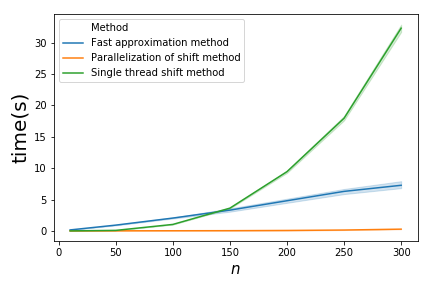
\includegraphics[width=0.48\textwidth]{figures/SNSruntimeSingleThread5_2.png}\label{fig:noarmal04} &  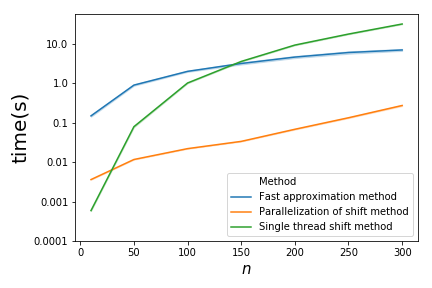
\includegraphics[width=0.48\textwidth]{figures/SNSruntimeLogSingleThread5_2.png}\label{fig:normal12} \\
  (a) & (b)
  \end{tabular}
  \caption{{\bf Run time requirements}. Experiment with $x^{A} \sim \mathcal{N}(5.0,1)$ and $x^{B} \sim \mathcal{N}(5.2,1)$. We plotted the required runtime, as wall time, as a function of the number of discretization windows, $n_w$, where (a) is on the normal-scale, and (b) is on the log-scale..\label{fig:runtime1}}
\end{figure}

\begin{figure}[H]
  \centering
  \begin{tabular}{cc}
  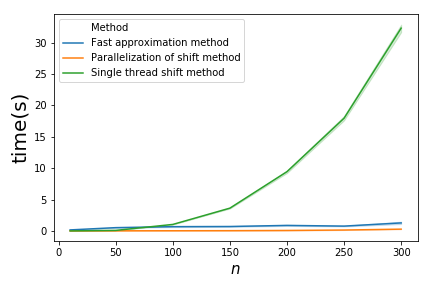
\includegraphics[width=0.48\textwidth]{figures/SNSruntimeSingleThread6_0.png}\label{fig:noarmal04} &  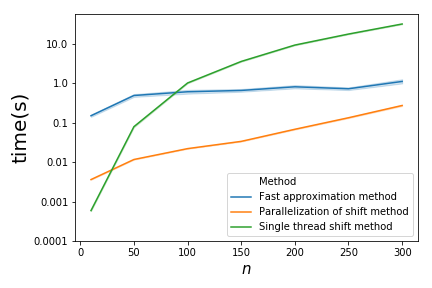
\includegraphics[width=0.48\textwidth]{figures/SNSruntimeLogSingleThread6_0.png}\label{fig:normal11} \\
  (a) & (b)
  \end{tabular}
  \caption{{\bf Run time requirements}. Experiment with $x^{A} \sim \mathcal{N}(5.0,1)$ and $x^{B} \sim \mathcal{N}(6.0,1)$. We plotted the required runtime, as wall time, as a function of the number of discretization windows, $n_w$, where (a) is on the normal-scale, and (b) is on the log-scale..\label{fig:runtime2}}
\end{figure}

In the figures above \ref{fig:runtime1} and \ref{fig:runtime2}, it's evident that the parallelized shift method is quicker than the fast approximation method. Even with a steelman argument, i.e., comparing where fast approximation method performs the best contra where parallelized shift method achieves the worst (that would be at $n=300$ in figure \ref{fig:runtime2}, the parallelized method is approximately $4.5$ times faster. This time difference would make a significant difference for experiments with many samples. For instance, the human genome has over 20.000 genes (samples), which, in this scenario (cohort of $n=300$ patients), would require a couple of hours runt-time instead of a workday.

\subsubsection{Time development of changes in discretization window $n_ w$ and set size $n$}
In the first test (Figure \ref{fig:runtime1}), $n=m=200$ and $n_{w} \in \mathbf{n_{w}}=[10,50,100,200]$, i.e., where $n_{w}$ is the variable. In the second test (figure \ref{fig:runtime2}), $n_{w}=100$ and $\mathbf{n}=\mathbf{m}=[50, 100,150,200,250]$, i.e., where $n,m$ is the variables. Both used as sample size of $n_{samples}=1$, i.e., only one $(\bf{x^{A}}, \bf{x^{B}})$ sample pair.

    \todo[inline]{Here we need the same types of test as we currently use, however, we need to include the series for the fastperm method, and shift the y-axis so it use a log-scale. Ideally you should also include error bands, \url{https://seaborn.pydata.org/examples/errorband_lineplots.html}}



\begin{figure}[H]
  \centering
  \begin{tabular}{cc}
  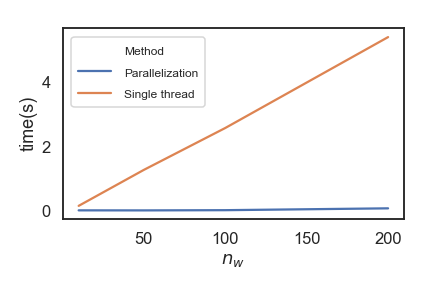
\includegraphics[width=0.48\textwidth]{figures/VarS.png}\label{fig:noarmal04} &  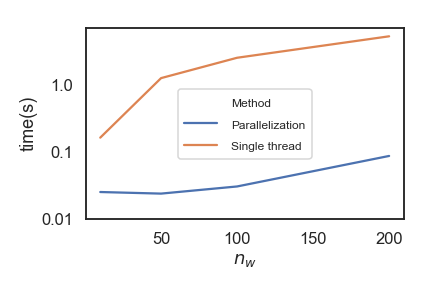
\includegraphics[width=0.48\textwidth]{figures/VarSLog.png}\label{fig:normal12} \\
  (a) & (b)
  \end{tabular}
  \caption{{\bf Run time requirements}. We plotted the required runtime, as wall time, as a function of the number of discretization windows, $n_w$, where (a) is on the normal-scale, and (b) is on the log-scale..\label{fig:runtime3}}
\end{figure}

\begin{figure}[H]
  \centering
  \begin{tabular}{cc}
  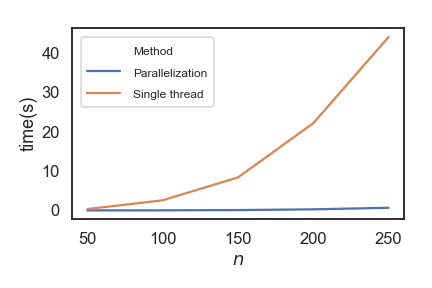
\includegraphics[width=0.48\textwidth]{figures/VarN.png}\label{fig:noarmal04} &  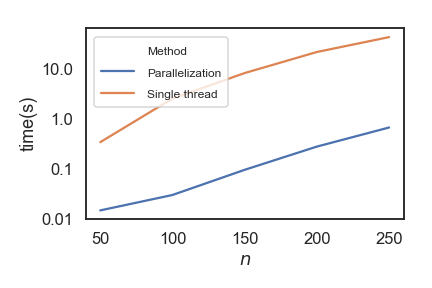
\includegraphics[width=0.48\textwidth]{figures/VarNLog.png}\label{fig:normal12} \\
  (a) & (b)
  \end{tabular}
  \caption{{\bf Run time requirements}. We plotted the required runtime, as wall time, as a function of the set size, $n$, where (a) is on the normal-scale, and (b) is on the log-scale.\label{fig:runtime4}}
\end{figure}

\todo[inline]{Should the text below be moved to the discussion section?}

In the first experiment, $n_{w}$ is the variable. Since $n_{w}$ only changes range which $s$ can take on values, i.e., $0 \leq s \leq s_{\rm max}$, and from section \ref{sec:calcBottleneck} it's described that the run time is governed by $\mathcal{O}(m\cdot (m+n)\cdot s_{\rm max})$, and with everything fixed except $n_{bin}$, the algorithm scale linearly with $\mathcal{O}(s_{\rm max})$, which is demonstrated in the Figure \ref{fig:runtime1}. What this means in practice is that if one would like to obtain a more accurate $p$-value, one could increase the number of windows $n_w$ without increasing runtime severely–since it only scales linearly.
In the second run time experiment, $n,m$ are the variables. Here $m=n$, therefore, the run time is $\mathcal{O}(n \cdot 2n)=\mathcal{O}(n^{2})$. This is demonstrated experimentally, see Figure \ref{fig:runtime2}.
In both cases, the parallelized version has almost constant run time, and this is because the GPU calculates everything at the same speed until it reaches its max capacity. If that would be the case, one has to re-load the GPU, which would require additional time. Hence, for more massive datasets, the GPU plot would look more like a step-function. 

\subsection{Relative error to the $t$-test test: The test is performed for the shift method, fast approximation method, and Mann-Whitney $u$-test.}

    \todo[inline]{Here we need the same types of test as we currently use, however, we need to include the series for the fastperm method, as well as a Mann-Witney U-test. Y-axis should be logged, and the error labels should be marked with absolute errors.}
    
The experiments performed here use the same data used in section \ref{sec:runtime1}. However, here, the relative error of the $p$-value compared with the $t$-test is tested, i.e.,  $\Delta p _{rel} = \frac{|p^{*}-p_{t}|}{p_{t}}$. Recall, that for each set-size $n \in \mathbf{n}$, taking 50 samples (i.e., 50 $p$-values), hence 50 relative errors for each box in the box-plot below.

\begin{figure}[H]
  \centering
  \begin{tabular}{cc}
  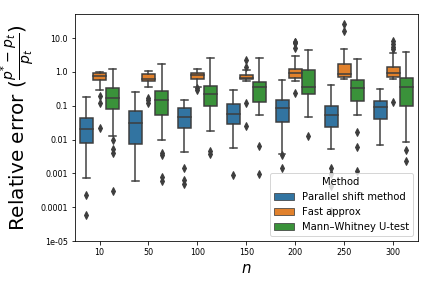
\includegraphics[width=0.45\textwidth]{figures/SNSfastPermMultipleBox5_2.png} &  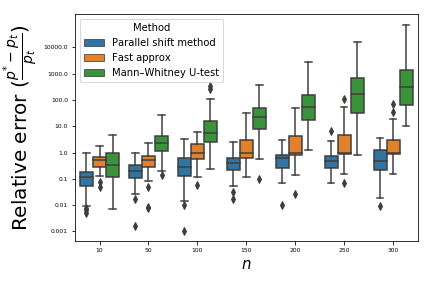
\includegraphics[width=0.45\textwidth]{figures/SNSfastPermMultipleBox6_0.png} \\
  (a) & (b)
  \end{tabular}
  \caption{{\bf Characterization of errors.} We plotted the relative error, on the log-scale, as a function of the set size, $n$, where (a) is the experiment with $x^{A} \sim \mathcal{N}(5.0,1)$ and $x^{B} \sim \mathcal{N}(5.2,1)$, and (b) is the experiment with $x^{A} \sim \mathcal{N}(5.0,1)$ and $x^{B} \sim \mathcal{N}(6.0,1)$.\label{fig:relerror}}
\end{figure}

\subsection{Calibration test: Checking uniformity of $p$-values from the shift method, fast approximation method, Mann-Whitney $u$-test, and $t$-test.}

All plots below demonstrates $10000$ samples (i.e., 10000 $p$-values) where $x^A_i, x^B_i \stackrel{\text{iid}}{\sim}\mathcal{D}(\mu , \sigma)$ i.e. $\mathbf{x^A}, \mathbf{x^B}$ originates from the same distribution. Since the null hypothesis is true one would except uniform distribution of the the $p$-values, which is tested with these following plots.

\begin{figure}[H]
  \centering
  \begin{tabular}{ccc}
  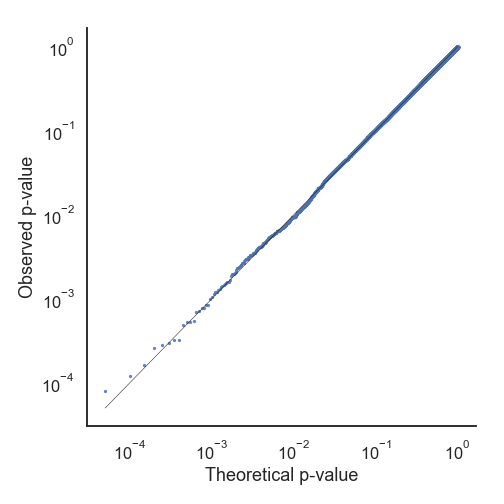
\includegraphics[width=0.33\textwidth]{figures/calibration/large_calibration/e_norm_0_1_50.png} & 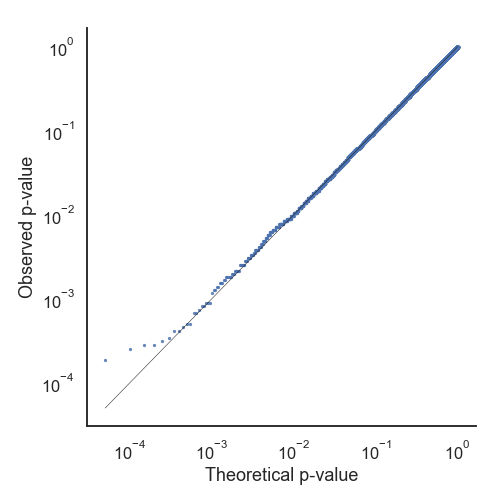
\includegraphics[width=0.33\textwidth]{figures/calibration/large_calibration/mw_norm_0_1_50.png} & 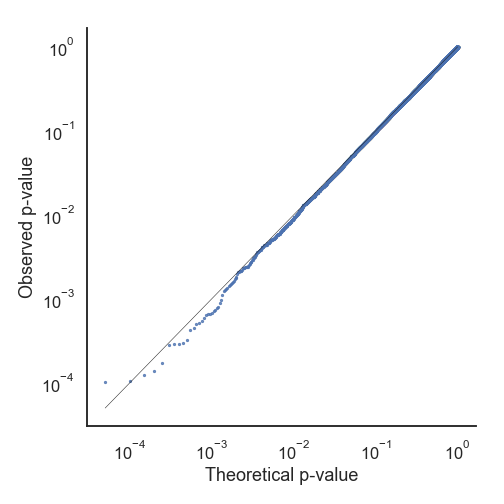
\includegraphics[width=0.33\textwidth]{figures/calibration/large_calibration/t_norm_0_1_50.png} \\
  (a) & (b) & (c)
  
  \end{tabular}
  \caption{{\bf Calibration plot.} Here $x^A_i, x^B_i \stackrel{\text{iid}}{\sim} \mathcal{N} (0 , 1)$ with set sizes $|x^A_i| = |x^B_i|=20$, where (a) parallelized exact test, (b) Mann-Whitney $u$-test, and (c) $t$-test.\label{fig:relerror}}
\end{figure}

\begin{figure}[H]
  \centering
  \begin{tabular}{ccc}
  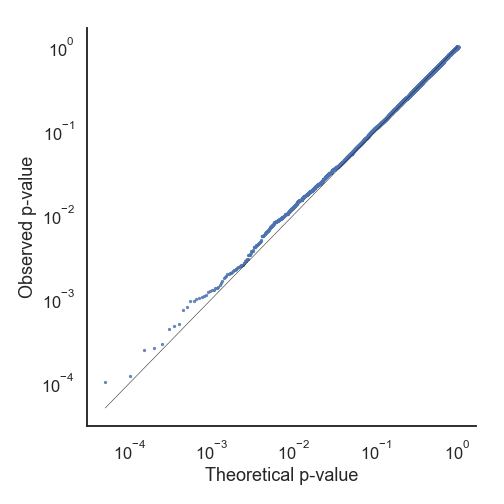
\includegraphics[width=0.33\textwidth]{figures/calibration/large_calibration/e_Lnorm_0_1_50.png} & 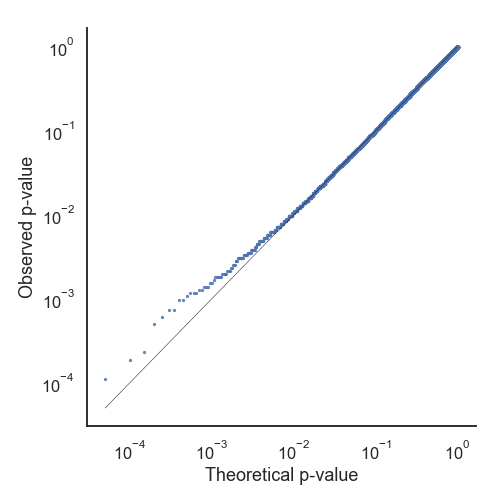
\includegraphics[width=0.33\textwidth]{figures/calibration/large_calibration/mw_Lnorm_0_1_50.png} & 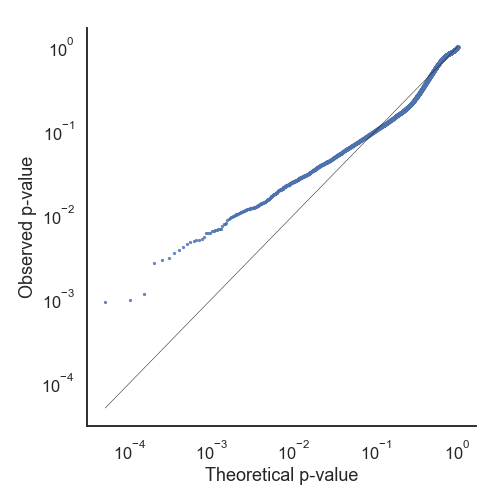
\includegraphics[width=0.33\textwidth]{figures/calibration/large_calibration/t_Lnorm_0_1_50.png} \\
  (a) & (b) & (c)
  
  \end{tabular}
  \caption{{\bf Calibration plot.} Here $x^A_i, x^B_i \stackrel{\text{iid}}{\sim} log\mathcal{N} (0 , 2)$ with set sizes $|x^A_i| = |x^B_i|=20$, where (a) parallelized exact test, (b) Mann-Whitney $u$-test, and (c) $t$-test.\label{fig:relerror}}
\end{figure}


\begin{comment}



\begin{figure}[H]
  \centering
  \begin{tabular}{cc}
  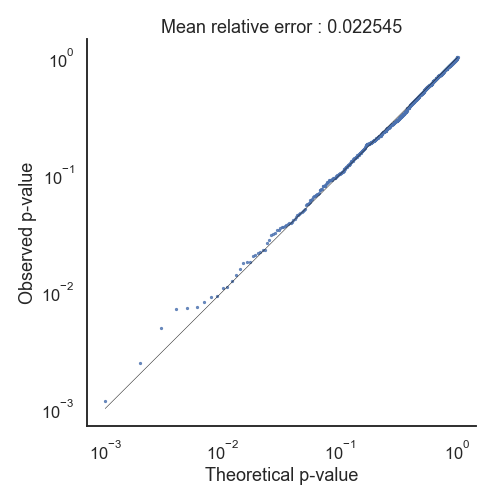
\includegraphics[width=0.45\textwidth]{figures/calibration/norm_5_1_s10/e.png} & 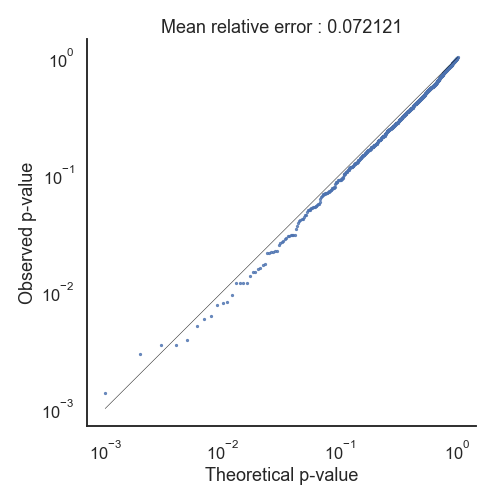
\includegraphics[width=0.45\textwidth]{figures/calibration/norm_5_1_s10/f.png} \\
  (a) & (b) \\
  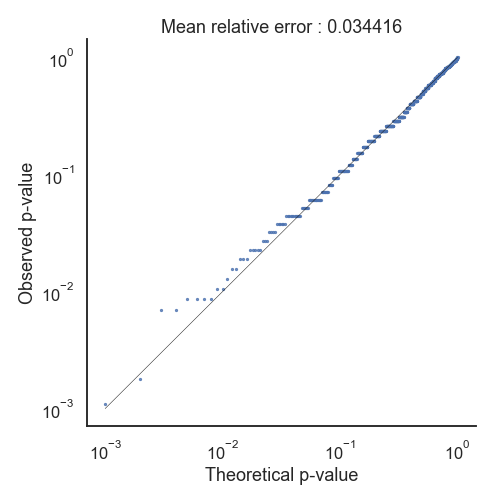
\includegraphics[width=0.45\textwidth]{figures/calibration/norm_5_1_s10/mw.png} &  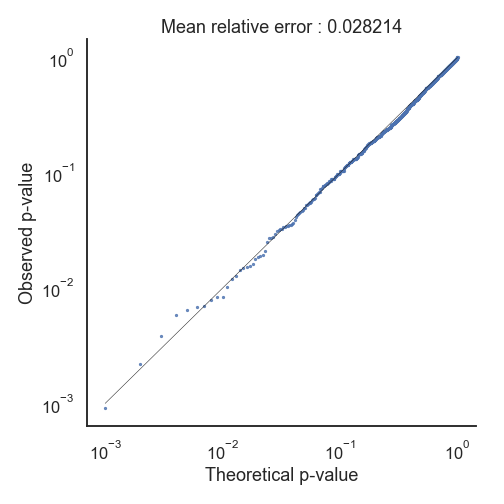
\includegraphics[width=0.45\textwidth]{figures/calibration/norm_5_1_s10/t.png} \\
  (c) & (d)
  \end{tabular}
  \caption{{\bf Calibration plot.} Here $x^A_i, x^B_i \stackrel{\text{iid}}{\sim} \mathcal{N}(5 , 1)$ with set sizes $|x^A_i| = |x^B_i|=10$, where (a) parallelized exact test, (b) fast approximation exact test, (c) Mann-Whitney $u$-test, and (d) $t$-test .\label{fig:relerror}}
\end{figure}

\begin{figure}[H]
  \centering
  \begin{tabular}{cc}
  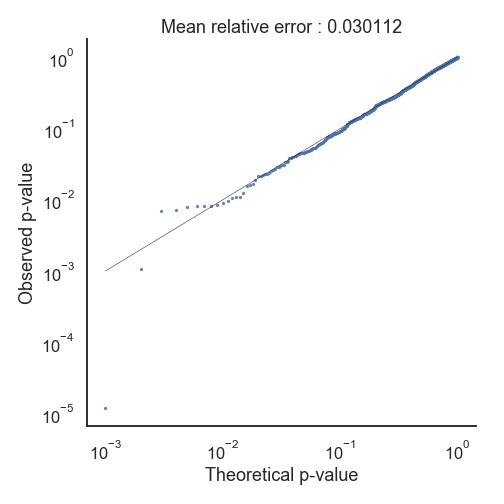
\includegraphics[width=0.45\textwidth]{figures/calibration/norm_5_1_s200/e.png} & 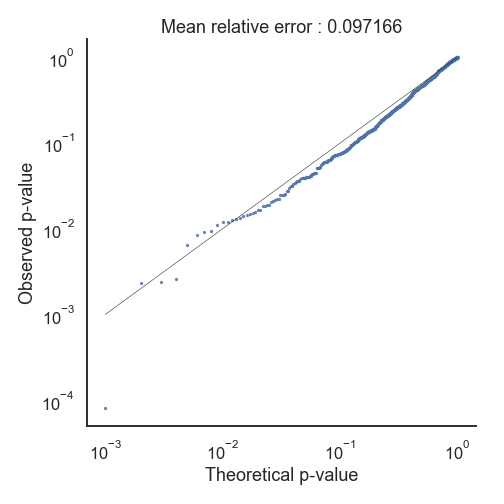
\includegraphics[width=0.45\textwidth]{figures/calibration/norm_5_1_s200/f.png} \\
  (a) & (b) \\
  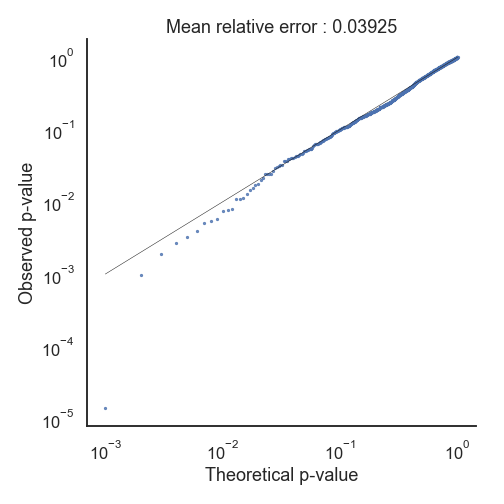
\includegraphics[width=0.45\textwidth]{figures/calibration/norm_5_1_s200/mw.png} &  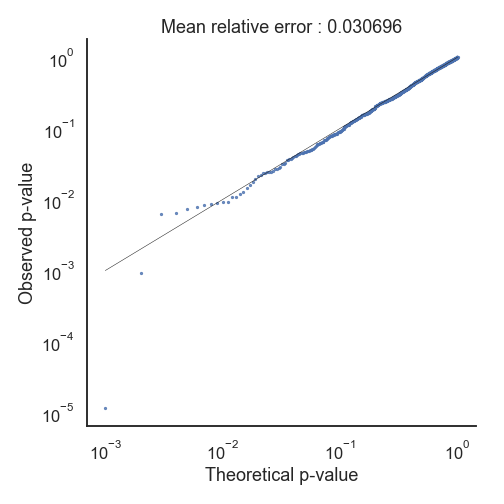
\includegraphics[width=0.45\textwidth]{figures/calibration/norm_5_1_s200/t.png} \\
  (c) & (d)
  \end{tabular}
  \caption{{\bf Calibration plot.} Here $x^A_i, x^B_i \stackrel{\text{iid}}{\sim} \mathcal{N}(5 , 1)$ with set sizes $|x^A_i| = |x^B_i|=200$, where (a) parallelized exact test, (b) fast approximation exact test, (c) Mann-Whitney $u$-test, and (d) $t$-test .\label{fig:relerror}}
\end{figure}

\begin{figure}[H]
  \centering
  \begin{tabular}{ccc}
  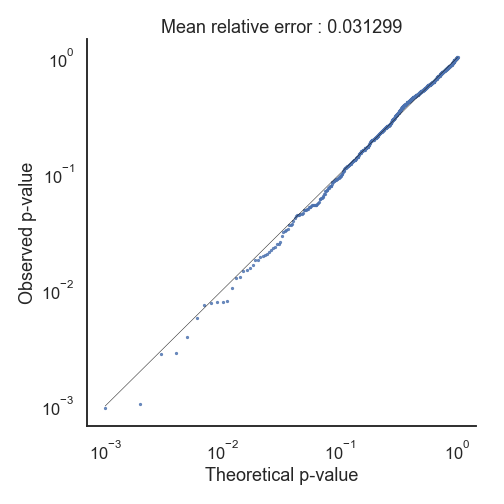
\includegraphics[width=0.33\textwidth]{figures/calibration/beta_2_5_s10/e.png} & 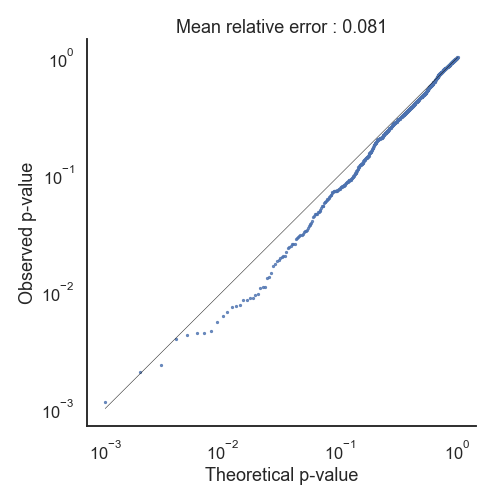
\includegraphics[width=0.33\textwidth]{figures/calibration/beta_2_5_s10/f.png} & 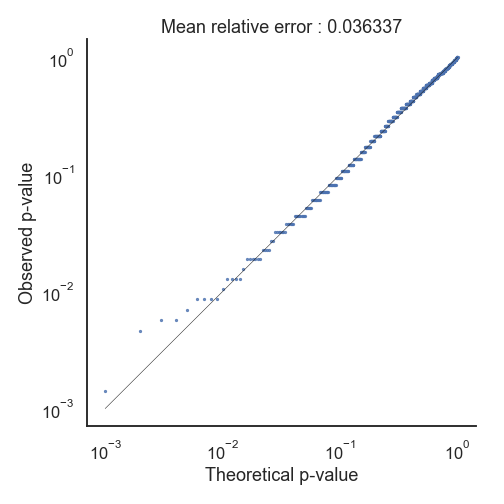
\includegraphics[width=0.33\textwidth]{figures/calibration/beta_2_5_s10/mw.png} \\
  (a) & (b) & (c)
  
  \end{tabular}
  \caption{{\bf Calibration plot.} Here $x^A_i, x^B_i \stackrel{\text{iid}}{\sim} \beta (2 , 5)$ with set sizes $|x^A_i| = |x^B_i|=10$, where (a) parallelized exact test, (b) fast approximation exact test, and (c) Mann-Whitney $u$-test.\label{fig:relerror}}
\end{figure}

\begin{figure}[H]
  \centering
  \begin{tabular}{ccc}
  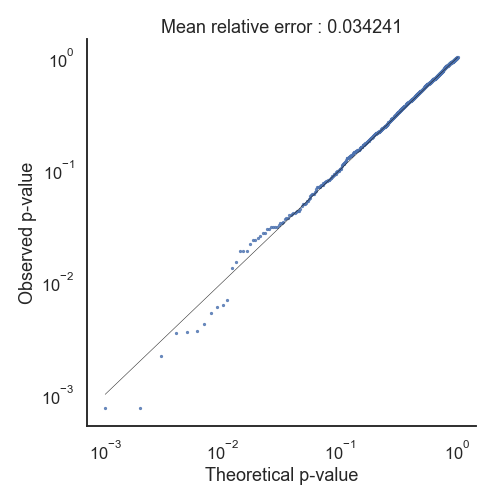
\includegraphics[width=0.33\textwidth]{figures/calibration/beta_2_5_s200/e.png} & 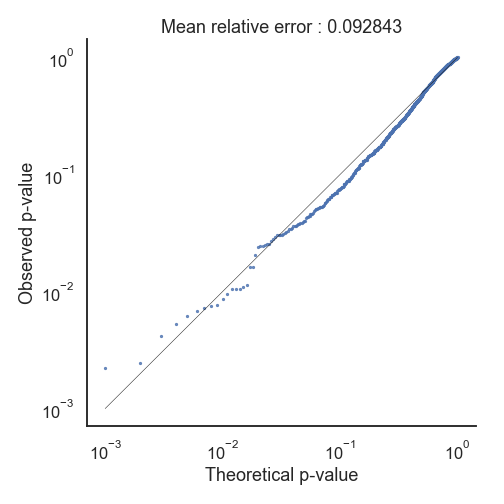
\includegraphics[width=0.33\textwidth]{figures/calibration/beta_2_5_s200/f.png} & 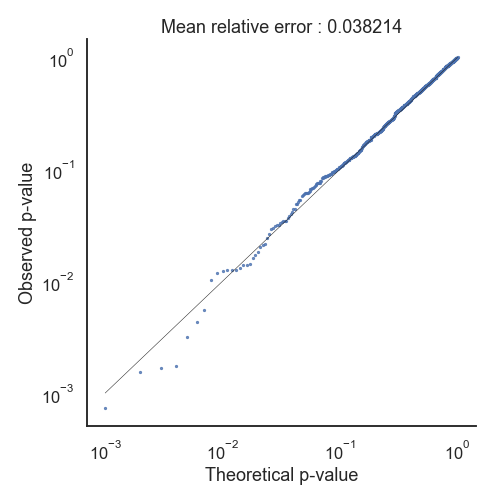
\includegraphics[width=0.33\textwidth]{figures/calibration/beta_2_5_s200/mw.png} \\
  (a) & (b) & (c)
  
  \end{tabular}
  \caption{{\bf Calibration plot.} Here $x^A_i, x^B_i \stackrel{\text{iid}}{\sim} \beta (2 , 5)$ with set sizes $|x^A_i| = |x^B_i|=200$, where (a) parallelized exact test, (b) fast approximation exact test, and (c) Mann-Whitney $u$-test.\label{fig:relerror}}
\end{figure}

\end{comment}



\begin{comment}

The distributions used are $A \sim \mathcal{N}(0,1)$ and $B \sim \mathcal{N}(\mu,1)$ where $\boldsymbol{\mu} = \{0.4, 1.2 \}$ (i.e., performing $|\boldsymbol{\mu}|=11$ experiments). The sizes of both $A$ and $B$ is $100$ (i.e., $|A|=|B|=100$), a sampling which was repeated for $70$ different seeds. For each $\mu \in \boldsymbol{\mu}$ (i.e., for each experiment), different numbers of windows $\boldsymbol{n_{w}}=\{10,15,20,\ldots,60\}$ are tested for the exact test and testing a total of $|\boldsymbol{n_{w}}|=21$ number of windows per experiment. For each number of windows (i.e., $n_{w} \in \boldsymbol{n_{w}}$), $70$ $p$-values are calculated (one for each of the $70$ samples) for the exact test and $t$-test, to then compute the relative error, i.e.,  $\Delta p _{rel} = \frac{p_{e}-p_{t}}{p_{t}}$. The idea is that the mean $\overline{\Delta p _{rel}}$ and the variance should decreases with increasing number of windows $n_{w}$. Which it indeed does, demonstrated in Figure \ref{fig:relerror}.

\end{comment}

\subsection{Implementation}
A python 3.6 implementation implementing the above algorithm is made available under an Apache 2.0 license. The implementation and all results of this paper are available in reproducible form from GitHub\footnote{\href{https://github.com/statisticalbiotechnology/parallelizedShiftExactPermTest}{https://github.com/statisticalbiotechnology/parallelizedShiftExactPermTest}}.

\section{Discussion}

Here we have described a parallellized dynamic programming method to perform permutation tests. We have demonstrated that it is faster and more accurate than the sampling based methods. We note that several studies are dependent on normal approximations of nonparametric tests such as the Mann-Witney U test. blabla

Use cases?

The discretization strategy ...

Future improvements, Handle missing values ...

\begin{comment}
\begin{figure}[H]
\centering
\begin{tikzpicture}[set style={{help lines}+=[dashed]}, xscale=1.7, yscale=0.75]
\draw[style=help lines] (-1,1) grid +(4,6);
\draw                   (0,5) grid +(1,1);
\node  at  (0.5, 5.5) {$1$};


\draw                   (1,3) grid +(1,1);
\node  at  (1.5,3.5) {$N_{old}(2,1)$};

\draw                   (2,1) grid +(1,1);
\node  at  (2.5,1.5) {$N_{old}(4,2)$};

\draw                   (2,5) grid +(1,1);
\node  at  (2.5,5.5) {$N_{old}(0,2)$};


%
\draw[style=help lines] (4,1) grid +(3,5);
\draw                   (5,3) grid +(1,1);
\node  at  (5.5,3.5) {$N_{new}(2,1)$};

\draw                   (4,5) grid +(1,1);
\node  at  (4.5,5.5) {$1$};
\draw                   (6,1) grid +(1,1);
\node  at  (6.5,1.5) {$N_{new}(4,2)$};

\draw                   (6,5) grid +(1,1);
\node  at  (6.5,5.5) {$N_{new}(0,2)$};


%------------------------------------------------------
% red1
\draw   [red,very thick,dashed,->]   (3,5.5) -- (6,5.5);
\draw   [red,very thick,->]   (1,5.5) -- (5,3.5);
\draw   [red,very thick,->]   (2,3.5) -- (5,3.5);
\draw   [red,very thick,->]   (3,1.5) -- (6,1.5);
\draw   [red,very thick,->]   (2,3.5) -- (6,1.5);

% black
\draw   [black,very thick,-]   (-1, 7) -- (3,7);
\draw   [black,very thick,-]   (-1, 6) -- (3,6);

\draw   [black,very thick,-]   (-1,1) -- (-1,7);
\draw   [black,very thick,-]   (0, 1) -- (0,7);

\draw   [black,very thick,-]   (-1, 1) -- (0,1);
\draw   [black,very thick,-]   (-1, 2) -- (0,2);
\draw   [black,very thick,-]   (-1, 3) -- (0,3);
\draw   [black,very thick,-]   (-1, 4) -- (0,4);
\draw   [black,very thick,-]   (-1, 5) -- (0,5);

\draw   [black,very thick,-]   (3,6) -- (3,7);
\draw   [black,very thick,-]   (2,6) -- (2,7);
\draw   [black,very thick,-]   (1,6) -- (1,7);

\draw   [black,very thick,-]   (-1,7) -- (0,6);


% circles
\draw  [fill=white, dashed] (3.5,5.5) circle (0.3);
\node  at  (3.5,5.5) {1};
\draw  [fill=white] (3.5,4.25) circle (0.3);
\node  at  (3.5,4.25) {2};
\draw  [fill=white] (3.5,2.8) circle (0.3);
\node  at  (3.5,2.8) {4};
\draw  [fill=white] (3.5,3.5) circle (0.3);
\node  at  (3.5,3.5) {3};
\draw  [fill=white] (3.5,1.5) circle (0.3);
\node  at  (3.5,1.5) {5};


% Heading
\node  at  (1.5,7.5) {\large $N_{old}$};
\node  at  (5.5,7.5) {\large $N_{new}$};

\node  at  (-0.2,6.65) {\large $j$};
\node  at  (0.5,6.5) {\large $0$};
\node  at  (1.5,6.5) {\large $1$};
\node  at  (2.5,6.5) {\large $2$};

\node  at  (-0.8,6.40) {\large $s$};
\node  at  (-0.5,5.50) {\large $0$};
\node  at  (-0.5,4.50) {\large $1$};
\node  at  (-0.5,3.50) {\large $2$};
\node  at  (-0.5,2.50) {\large $3$};
\node  at  (-0.5,1.50) {\large $4$};


% -------- Fill numbers -----------
\end{tikzpicture}

\caption{Illustration of the recursive computations of three entries of $N_{new}$ from elements in $N_{old}$.}\label{fig:recursion}
\end{figure}

\end{comment}


\begin{itemize}
\item Persuade the reader that the suggested algorithm provides an added value in particular situations!
\end{itemize}

\bibliographystyle{ieeetr}
\bibliography{refs}
\end{document}